This project attempts to deliver on a haptics focused terrain editing experience first and foremost. The overaching approach was to first establish a reliable coupling via a virtual proxy to Unity's physics system, and then create a proof of concept terrain editing tool which is driven by said proxy.

The three fundamental questions we had were as follows:

\begin{enumerate}
    \item How would we design a generic virtual coupling between Unity's physics engine and the Haply's force feedback mechanisms?
    \item How would we detect and render textures in realtime?
    \item How would we design the tool itself, with the main mode of interaction being through the Haply?
\end{enumerate}

\subsection{How would we design a generic virtual coupling between Unity's physics engine and the Haply's force feedback mechanisms?} \label{subsec:virtual-coupling}

We initially employed the Unity template obtained from the Haply GitLab repository as the foundation for our implementation. However, upon closer examination, it became evident that the forces applied were hardcoded, prompting us to adopt a PD controller model \cite{mathworksPID} facilitated by a virtual proxy (\textit{See \ref*{fig:virtual-coupling}}), as elaborated below.

In our implementation, we utilized Unity game objects, specifically one designated as the "\textbf{End Effector Actual}" to track the ideal positional data of the Haply, and another marked as the "\textbf{End Effector Representation}" equipped with a built-in sphere collider. This was to allow it to interact with Unity's physics engine. Subsequently, we established a PD controller relationship between these two entities. The underlying operational logic mandated the "\textbf{End Effector Representation}" to consistently attempt to minimize the euclidean distance between itself and the "\textbf{End Effector Actual}". This behavior was governed primarily by the proportional component of the PD controller, supplemented by the derivative component to offer additional smoothing (\textit{See \ref*{fig:virtual-coupling-a}}). In instances where the "\textbf{Representation}" detected any physical collisions, it directed the Haply to exert a force in the direction of the "\textbf{Representation}" from the "\textbf{Actual}" (\textit{See \ref*{fig:virtual-coupling-b}}). This would happen in parallel to the distance minimization attempts of the "\textbf{Representation}". Consequently, this establishment facilitated an adaptable virtual coupling mechanism, subject to the influence of Unity's physics engine via the intermediary proxy.

\begin{figure}[htbp]
    \centering
    \begin{subfigure}[b]{0.4\textwidth}
        \centering
        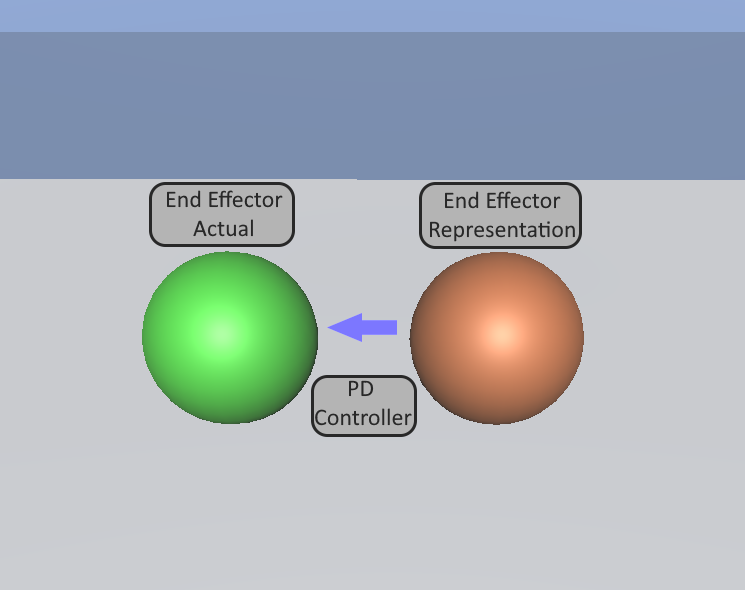
\includegraphics[width=\textwidth]{images/approach-virtual-coupling-a.png}
        \caption{PD controller moves Representation to Actual if there is no obstruction}
        \label{fig:virtual-coupling-a}
    \end{subfigure}
    \quad
    \quad
    \begin{subfigure}[b]{0.4\textwidth}
        \centering
        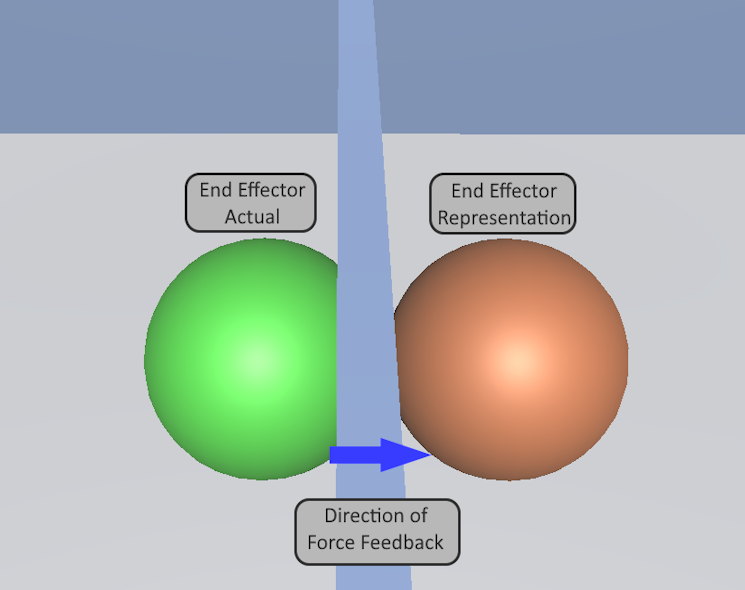
\includegraphics[width=\textwidth]{images/approach-virtual-coupling-b.png}
        \caption{Force Feedback Rendered if physics collision is detected}
        \label{fig:virtual-coupling-b}
    \end{subfigure}
    \caption{Virtual Coupling between Representation and Actual End Effector. Note that the \textbf{"End Effector Actual"} was never visualised in the tool itself.}
    \label{fig:virtual-coupling}
\end{figure}

Notably, while the direction vector was three-dimensional, only the X and Z components of this vector were translated to the Haply to render force feedback. The selected axes were simply an artifact of our design decision for editing on a terrain lying in the X-Z plane.

\subsection{How would we detect and render textures in realtime?} \label{subsec:texture-rendering}

Tangentially influenced by the research conducted by Li et al. (2010) \cite{li2010image}, we opted to leverage the inherent image data embedded within the texture for the application of small directional jitters. The procedural approach to texture rendering works by sampling a three by three pixel window beneath the end effector representation. Subsequently, grayscale conversion is applied to this sampled data, facilitating the extraction of pixel brightness values. The brightest pixels then exert the strongest forces away from itself. This mechanism imparts the perceptual impression of being coerced towards regions of lower luminosity, which can intuitively be mapped to "lower points" in the texture. Critically, this force modulation only manifests during end effector movement, thereby avoiding any undesirable tremors during static user positioning. By recalculating this tug force on a per-frame basis, an appreciable frequency modulation is introduced to the end effector, directly mirroring the texture's visual attributes (\textit{See \ref{fig:texture-rendering}}).

\begin{figure}[htbp]
    \centering
    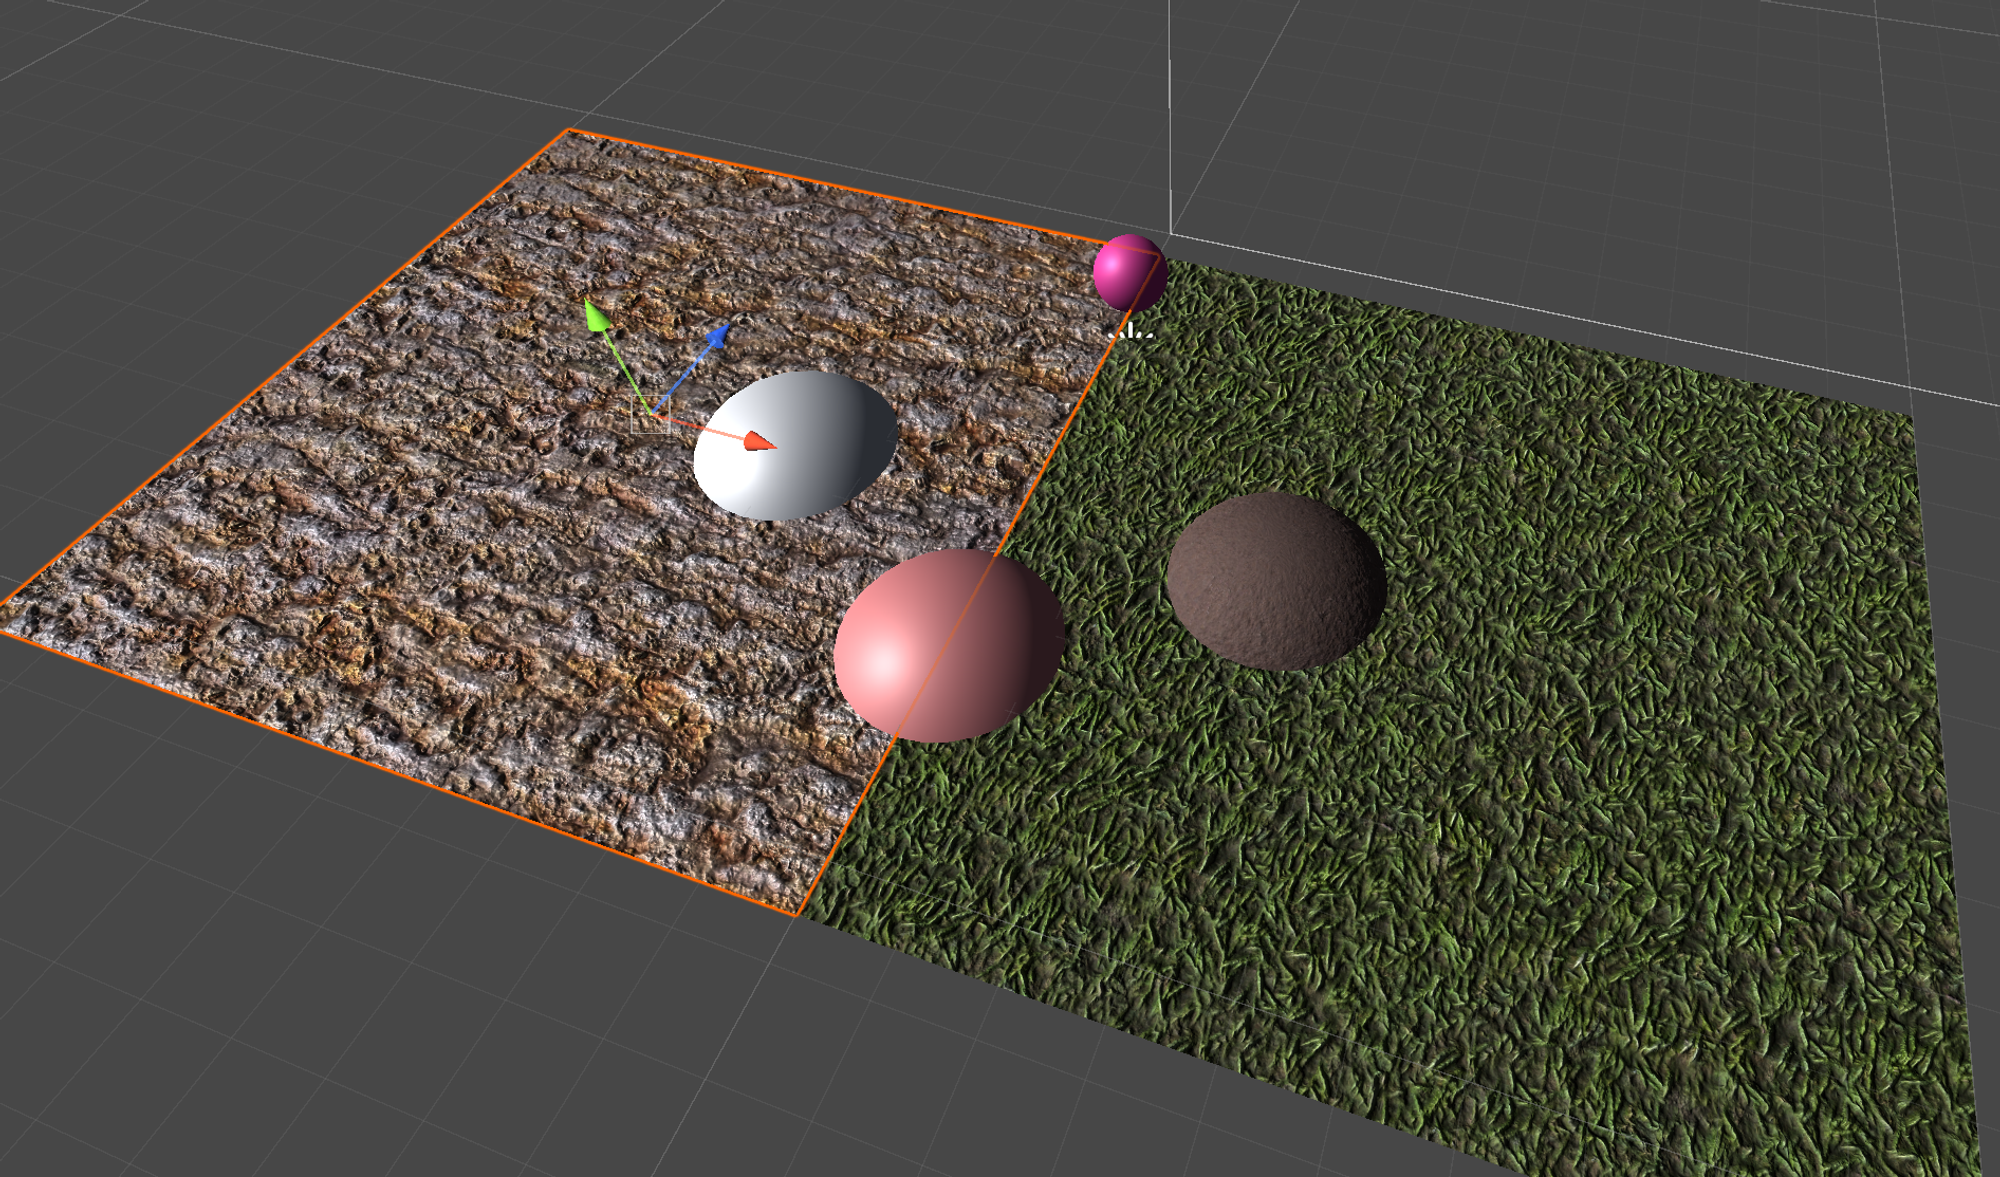
\includegraphics[width=0.8\textwidth]{images/approach-texture-rendering.png} 
    \caption{Two different textures providing different jittery sensations}
    \label{fig:texture-rendering}
\end{figure}

Although our initial goal was the utilization of heightmap data instead of the texture's pixel values, we found the latter approach yielded satisfactory outcomes during informal tests, prompting its adoption as the preferred methodology.

\subsection{How would we design the tool itself, with the main mode of interaction being through the Haply?} \label{subsec:terrain-painting}

Game engines typically offer a range of tools for terrain editing, which are primarily oriented towards editing within the editor environment rather than functioning during runtime. Consequently, it became necessary for us to reconstruct the fundamental components of a terrain editing tool within Unity, essentially embedding them as "game mechanics". This endeavor primarily involved leveraging Unity's Terrain game object \cite{unityterrain}, which is specially built to optimally encode localised texture and static object placement data. A straightforward user interface facilitates the selection among textures, objects, and an eraser tool, further categorized into sub-menus delineating texture types (e.g., grass, sand) and object variants (e.g., trees, rocks) (refer to Figure \ref{fig:terrain-painting}). The user can then designate their preferred object or texture through mouse interaction. Upon selection, the haply device acts akin to a virtual paintbrush, allowing object placement or texture painting at the location of the end effector. Activation of the painting action is achieved either through the stylus button integrated with Gen3 DIY devices or, alternatively, by utilizing the spacebar in cases where the stylus button is unavailable.

\begin{figure}[htbp]
    \centering
    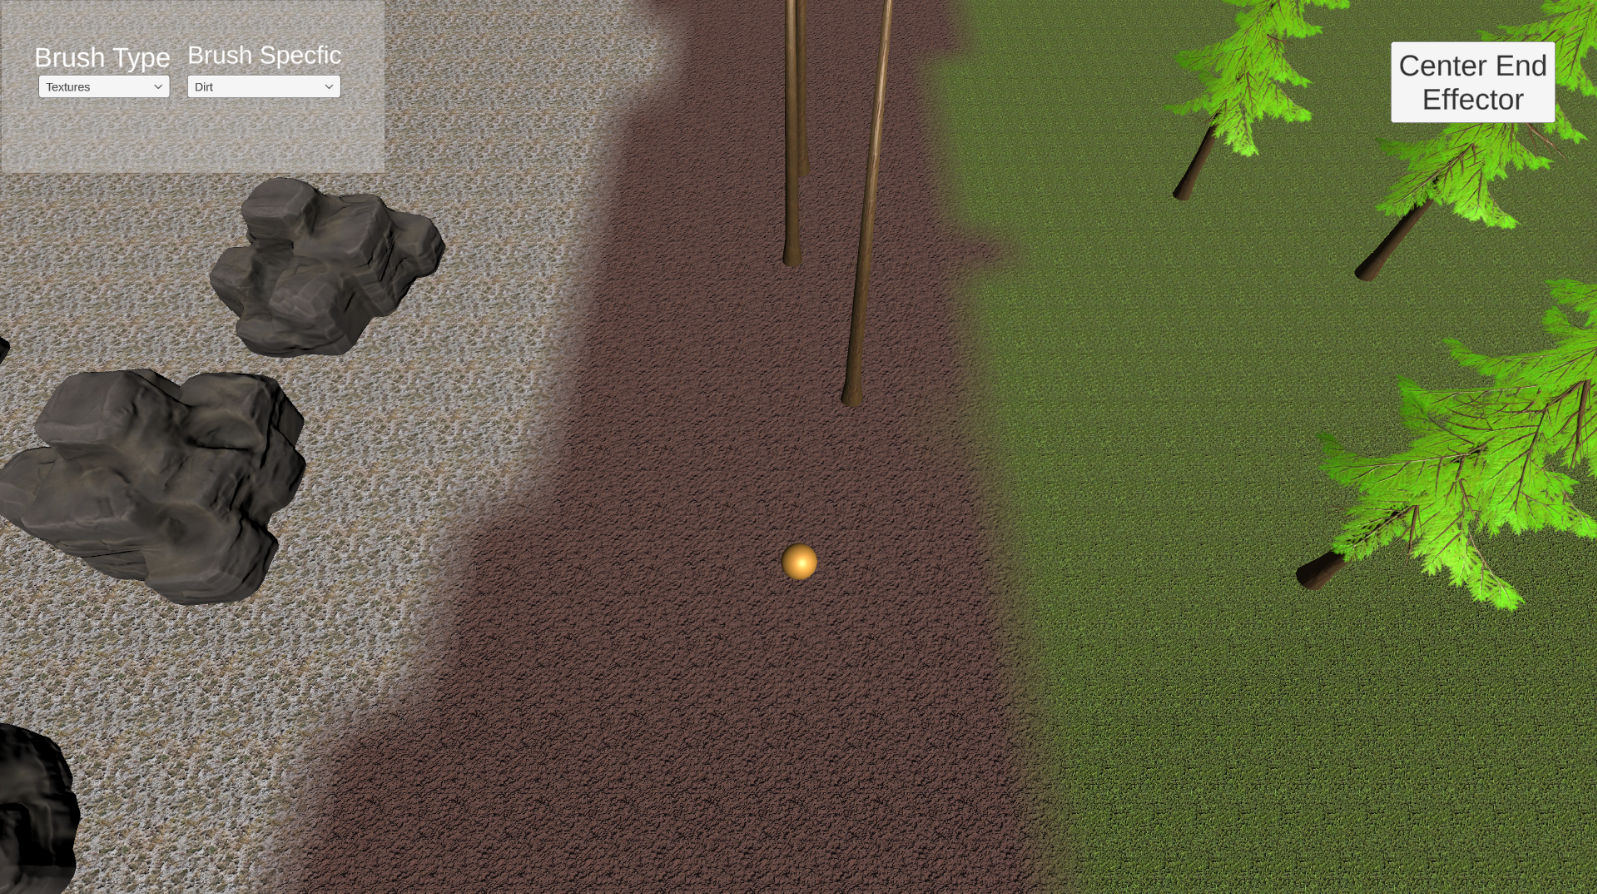
\includegraphics[width=0.8\textwidth]{images/approach-terrain-painter.png} 
    \caption{The final terrain painting interface}
    \label{fig:terrain-painting}
\end{figure}

The central utility of this approach lies in its capacity to provide users with tactile feedback with their interactions with the terrain in real-time. Objects impart a rigid collider-based resistance as a consequence of the virtual coupling (see Subsection \ref{subsec:virtual-coupling}), while textures provide haptic modulation based on their visual characteristics and behavior in accordance with haptic texture rendering principles (see Subsection \ref{subsec:texture-rendering}).
